\setAuthor{Eero Vaher}
\setRound{lahtine}
\setYear{2015}
\setNumber{G 10}
\setDifficulty{9}
\setTopic{Magnetism}

\prob{Laetud pendel}
Väike laetud kuulike massiga $m$ ja laenguga $q$ ripub venimatu pikkusega $l$ niidi otsas magnetväljas induktsiooniga $B$. Kuulike viiakse niiti sirgena hoides kõrgusele $H=\frac{7}{8}l$ ning lastakse siis lahti. Raskuskiirendus on $g$ ning magnetvälja suund on risti pendli võnketasandiga. Samuti on teada, et kehtib $q^2B^2l=\frac{3}{4}m^2g$. Milline on kuulikese trajektoor?

\begin{center}
\begin{resizebox}{0.5\linewidth}{!}{
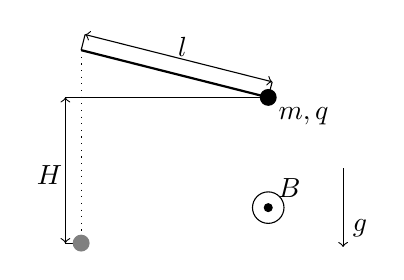
\begin{tikzpicture}
\newcommand{\x}{1.2*1.98}
\newcommand{\y}{-0.6}
\newcommand{\length}{{veclen(\x,\y)}}

\draw (\x,-2) circle (0.2) node [above right] {$B$};
\draw[fill=black] (\x, -2) circle (0.05);
\draw[->] (1.4*\x,-1.5) -- (1.4*\x,-2.5) node[above right] {$g$};

\draw[<->] (0.05,-0.05*\x/\y) -- (\x+0.05,\y-0.05*\x/\y);
\draw (0,0) -- (0.05,-0.05*\x/\y);
\draw (\x,\y) -- (\x+0.05,\y-0.05*\x/\y);
\draw[thick] (0,0) -- (\x,\y) node[below right] {$m,q$};
\draw[fill=black] (\x,\y) circle (0.1);
\node[above] at (\x/2+0.1,\y/2+0.1) {$l$};

\draw[<->] (-0.2,\y) -- (-0.2,-\length);
\draw (\x,\y) -- (-0.2,\y);
\draw (0,-\length) -- (-0.2,-\length);
\draw[dotted] (0,0) -- (0,-\length);
\draw[gray, fill=gray] (0,-\length) circle (0.1);
\node[left] at (0,-\length/2.5+\y) {$H~$};
\end{tikzpicture}}
\end{resizebox}
\end{center}

\hint
Kuulikesele mõjuvad raskusjõud, niidi pinge ning Lorentzi jõud. Kuulike püsib ringjoone kaare kujulisel trajektooril seni, kuni Lorentzi jõud ja niidi pinge ületavad ülejäänud jõudude niidisihilise komponendi. Vastav kriitiline nurk on leitav energia jäävuse seadusest ning jõudude tasakaalust.

\solu
Kuulikesele mõjuvad raskusjõud $F_g$, niidi pinge $T$ ning Lorentzi jõud $F_L$. Kuulike püsib ringjoone kaarekujulisel trajektooril seni, kuni sellele mõjuvate jõudude projektsioonid niidi sihile rahuldavad võrrandit $T+F_L-F_g\cos\alpha=F_k$, kus $\alpha$ on niidi kõrvalekaldenurk tasakaaluasendist ning $F_k$ on ringjoone kaarel püsimiseks tarvilik kesktõmbejõud. Kuulikese ringjoone kaarekujulisest trajektoorist kõrvalekaldumisel ei saa niit olla pinges. Järelikult pole kuulikese trajektoor enam ringjoone kaar juhul $F_L>F_g\cos\alpha+F_k$. Olgu $v$ kuulikese kiirus nurga $\alpha$ korral, mille saame leida energia jäävusest 
\[
\frac{mv^2}{2}=-mg\Delta h,
\]
kus $\Delta h=l\cos\alpha-l+H$ on kuulikese kõrguse muut. Järelikult 
\[
v=\sqrt{2g\left(l\cos\alpha-l+H\right)}=\sqrt{2gl\left(\cos\alpha-\frac{1}{8}\right)}
\]
ning lahendamist vajav võrrand on $qBv=mg\cos\alpha+\frac{mv^2}{l}$ ehk 
\[
qB\sqrt{2gl\left(\cos\alpha-\frac{1}{8}\right)}=mg\cos\alpha+2mg\left(\cos\alpha-\frac{1}{8}\right).
\]
Mõlemaid pooli ruutu võttes saame
\[
2q^2B^2gl\left(\cos\alpha-\frac{1}{8}\right)=m^2g^2\left(3\cos\alpha-\frac{1}{4}\right)^2.
\] 
Kuna $2q^2B^2l=\frac{3}{2}m^2g$, siis võime selle võrrandi viia kujule 
\[
\frac{3}{2}\cos\alpha-\frac{3}{16}=9\cos^2\alpha-\frac{3}{2}\cos\alpha+\frac{1}{16}.
\]
Saame ruutvõrrandi $9\cos^2\alpha-3\cos\alpha+\frac{1}{4}=0$ ehk $9\left(\cos\alpha-\frac{1}{6}\right)^2=0$. Kuna selle ruutvõrrandi kaks lahendit on võrdsed, siis kas $F_L\leq F_g\cos\alpha+F_k$ või $F_L\geq F_g\cos\alpha+F_k$ iga $\alpha$ korral. Vaadeldes juhtu $\cos\alpha=\frac{1}{8}$ näeme, et $F_L\leq F_g\cos\alpha+F_k$ ning järelikult on kuulikese trajektoor ringjoone kaar raadiusega $l$, mille otspunktide kõrgus tasakaaluasendist on $\frac{7}{8}l$.

\probeng{Charged pendulum}
A small charged ball of mass $m$ and charge $q$ is hanging at the end of a non-stretchable thread of length $l$ in a magnetic field of induction $B$. The ball is brought to a height $H=\frac{7}{8}l$ while holding the thread straight and then it is let free. The gravitational acceleration is $g$ and the direction of the magnetic field is perpendicular to the plane of the pendulum. It is also known that $q^2B^2l=\frac{3}{4}m^2g$ applies. What is the trajectory of the ball?
\begin{center}
\begin{resizebox}{0.5\linewidth}{!}{
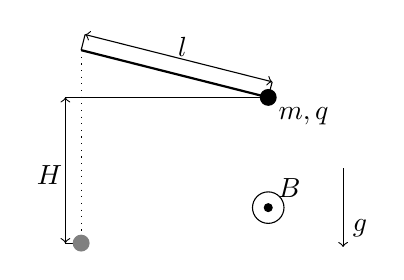
\begin{tikzpicture}
\newcommand{\x}{1.2*1.98}
\newcommand{\y}{-0.6}
\newcommand{\length}{{veclen(\x,\y)}}

\draw (\x,-2) circle (0.2) node [above right] {$B$};
\draw[fill=black] (\x, -2) circle (0.05);
\draw[->] (1.4*\x,-1.5) -- (1.4*\x,-2.5) node[above right] {$g$};

\draw[<->] (0.05,-0.05*\x/\y) -- (\x+0.05,\y-0.05*\x/\y);
\draw (0,0) -- (0.05,-0.05*\x/\y);
\draw (\x,\y) -- (\x+0.05,\y-0.05*\x/\y);
\draw[thick] (0,0) -- (\x,\y) node[below right] {$m,q$};
\draw[fill=black] (\x,\y) circle (0.1);
\node[above] at (\x/2+0.1,\y/2+0.1) {$l$};

\draw[<->] (-0.2,\y) -- (-0.2,-\length);
\draw (\x,\y) -- (-0.2,\y);
\draw (0,-\length) -- (-0.2,-\length);
\draw[dotted] (0,0) -- (0,-\length);
\draw[gray, fill=gray] (0,-\length) circle (0.1);
\node[left] at (0,-\length/2.5+\y) {$H~$};
\end{tikzpicture}}
\end{resizebox}
\end{center}

\hinteng
Gravity forces, the tension of the thread and the Lorentz force are applied to the ball. The ball stays in the circle’s arc shaped trajectory as long as the Lorentz force and the tension of the thread surpass the thread-directional components of the rest of the forces. The corresponding critical angle can be found through the conservation of energy and the force balance.

\solueng
The ball is affected by the gravity force $F_g$, thread’s tension $T$ and the Lorentz force $F_L$. The ball stays on the circle’s arc-shaped trajectory until the projections of the forces applied to it that are to the thread’s direction satisfy the equation $T+F_L-F_g\cos\alpha=F_k$ where $\alpha$ is the angle of deflection from the equilibrium position and $F_k$ is the necessary centripetal force to stay on the circle’s arc. The thread cannot be tense when the ball strays away from the circle’s arc-shaped trajectory. Therefore the ball’s trajectory is no longer a circle’s arc when $F_L>F_g\cos\alpha+F_k$. Let $v$ be the ball’s velocity for the angle $\alpha$ which we can find from the conversation of energy $\frac{mv^2}{2}=-mg\Delta h$, where $\Delta h=l\cos\alpha-l+H$ is the ball’s height change. Therefore 
\[
v=\sqrt{2g\left(l\cos\alpha-l+H\right)}=\sqrt{2gl\left(\cos\alpha-\frac{1}{8}\right)}
\]
and the equation needed to be solved is $qBv=mg\cos\alpha+\frac{mv^2}{l}$, meaning
\[
qB\sqrt{2gl\left(\cos\alpha-\frac{1}{8}\right)}=mg\cos\alpha+2mg\left(\cos\alpha-\frac{1}{8}\right).
\]
Squaring both sides we get
\[
2q^2B^2gl\left(\cos\alpha-\frac{1}{8}\right)=m^2g^2\left(3\cos\alpha-\frac{1}{4}\right)^2.
\]
Because $2q^2B^2l=\frac{3}{2}m^2g$ we can express this equation as $\frac{3}{2}\cos\alpha-\frac{3}{16}=9\cos^2\alpha-\frac{3}{2}\cos\alpha+\frac{1}{16}$. We get a quadratic equation $9\cos^2\alpha-3\cos\alpha+\frac{1}{4}=0$, meaning $9\left(\cos\alpha-\frac{1}{6}\right)^2=0$. Because the two solutions of this quadratic equations are equal then either $F_L\leq F_g\cos\alpha+F_k$ or $F_L\geq F_g\cos\alpha+F_k$ for each $\alpha$. Observing the case $\cos\alpha=\frac{1}{8}$ we see that $F_L\leq F_g\cos\alpha+F_k$ and therefore trajectory of the ball is a circle’s arc of radius $l$. The height of the arcs ends from the equilibrium position is $\frac{7}{8}l$.
\probend